\documentclass[a4paper,11pt,english]{report}
\newenvironment{packed_enum}{
\begin{itemize}
  \setlength{\itemsep}{1pt}
  \setlength{\parskip}{0pt}
  \setlength{\parsep}{0pt}
}{\end{itemize}}

\setlength{\parskip}{\baselineskip}
\usepackage[T1]{fontenc}
\usepackage[utf8]{inputenc}
\setcounter{secnumdepth}{3}
\setcounter{tocdepth}{3}
\usepackage{color}
\usepackage{array}
\usepackage{longtable}
\usepackage{multirow}
\usepackage{setspace}
\usepackage{hyperref}
\makeatletter
\usepackage{fancyhdr}
\usepackage{geometry}
\pagestyle{fancy}
\usepackage{afterpage}
\usepackage{framed}


%
%--------------------   start of the 'preamble'
%
\usepackage{graphicx,amssymb,amstext,amsmath}
\usepackage{listings}
\usepackage{color, colortbl}
\lstset{numbers=left, stepnumber=1, basicstyle=\scriptsize,}

%
%%    homebrew commands -- to save typing
\newcommand\comp{\textsl{The Companion}}
\newcommand\nss{\textsl{Not so Short}}
\newcommand{\noun}[1]{\textsc{#1}}

\definecolor{firebrick}{rgb}{0.98,0.15,0.04}
\definecolor{gold}{rgb}{1,0.83,0}
\definecolor{olive}{rgb}{0.49,0.89,0.1}
\definecolor{red3}{rgb}{1,0,0}
\definecolor{orangered}{rgb}{1,0.27,0}
\definecolor{lightgold}{rgb}{1,0.93,0.55}
\definecolor{chartreuse3}{rgb}{0.4,0.8,0}

\definecolor{olivedrab3}{rgb}{0.78,0.93,0.11}
\definecolor{goldenrod1}{rgb}{1,0.63,0}
\definecolor{yellow}{rgb}{0.78,0.93,0.11}
\setcounter{tocdepth}{2}
\providecommand{\tabularnewline}{\\}
\makeatother

%----------------------------------------------------------------------------------------
%	TITLE PAGE
%----------------------------------------------------------------------------------------

\newcommand*{\titleGM}{\begingroup % Create the command for including the title page in the document
\hbox{ % Horizontal box
\hspace*{0.2\textwidth} % Whitespace to the left of the title page
\rule{1pt}{\textheight} % Vertical line
\hspace*{0.05\textwidth} % Whitespace between the vertical line and title page text
\parbox[b]{0.75\textwidth}{ % Paragraph box which restricts text to less than the width of the page

{\noindent\Huge\bfseries Prescriptions  \\[0.5\baselineskip]  Management
 \\[0.5\baselineskip]  
}\\[2\baselineskip] % Title


\vspace{0.5\textheight}
%\vspace{0.2\textheight} % Whitespace between the title block and the publisher
%{\noindent  }{\Large \textsc{Olga Dzięgielewska\\[0.5\baselineskip] Marcin Klepaczka\\[0.5\baselineskip] %Andrzej Rybczak\\[0.5\baselineskip] Jan Szajda}} % Author name % Publisher and logo
%\vspace{0.1\textheight} % Whitespace between the title block and the publisher
\begin{flushright}
\includegraphics[scale=0.5]{"plaq"}
{\noindent  }{\\[0.3\baselineskip] \textsc{Wrocław, 2014}} 
\end{flushright}
}}

\endgroup}


%
%---------------------   end of the 'preamble'
%
\begin{document}
%-----------------------------------------------------------
\chead{}
\rhead{\includegraphics[scale=0.1]{"plaq"}}
\lfoot{}
\cfoot{\thepage}
\rfoot{}


%\maketitle
\thispagestyle{empty}
\titleGM

\chapter*{Authors}
\begin{itemize}

\item[] Zbginiew \textsc{Dobosiewicz}
\item[] Olga \textsc{Dzięgielewska} 
\item[] Michał \textsc{Kaczmarek} 
\item[] Paweł \textsc{Kędzia} 
\item[] Marcin \textsc{Klepaczka} 
\item[] Krystian \textsc{Krakowiak}
\item[] Piotr \textsc{Lipiak} 
\item[] Maciej \textsc{Niemczyk} 
\item[] Paweł \textsc{Nużka} 
\item[] Bartłomiej \textsc{Paciorek}
\item[] Bartosz \textsc{Piwowarski}
\item[] Jakub \textsc{Płaskonka} 
\item[] Mateusz \textsc{Płatek} 
\item[] Andrzej \textsc{Rybczak} 
\item[] Jan  \textsc{Szajda}
\end{itemize}

  
%-----------------------------------------------------------
\lhead[]{\textit{Prescriptions management: Contents }}
%-----------------------------------------------------------
\tableofcontents

% odstepy pomiedzy liniami na 1.

%-----------------------------------------------------------

\onehalfspacing



%\chapter{\noun{Purpose}   }

The purpose of this plan is to improve security and ensure the confidentiality, integrity, and availability of data in the Institute of Computer Security.

The purpose of this plan is to improve security and ensure the confidentiality, integrity, and availability of data in the Institute of Computer Security.

The purpose of this plan is to improve security and ensure the confidentiality, integrity, and availability of data in the Institute of Computer Security.

The purpose of this plan is to improve security and ensure the confidentiality, integrity, and availability of data in the Institute of Computer Security.

The purpose of this plan is to improve security and ensure the confidentiality, integrity, and availability of data in the Institute of Computer Security.

The purpose of this plan is to improve security and ensure the confidentiality, integrity, and availability of data in the Institute of Computer Security.

The purpose of this plan is to improve security and ensure the confidentiality, integrity, and availability of data in the Institute of Computer Security.

The purpose of this plan is to improve security and ensure the confidentiality, integrity, and availability of data in the Institute of Computer Security.

The purpose of this plan is to improve security and ensure the confidentiality, integrity, and availability of data in the Institute of Computer Security.

The purpose of this plan is to improve security and ensure the confidentiality, integrity, and availability of data in the Institute of Computer Security.

The purpose of this plan is to improve security and ensure the confidentiality, integrity, and availability of data in the Institute of Computer Security.

The purpose of this plan is to improve security and ensure the confidentiality, integrity, and availability of data in the Institute of Computer Security.

The purpose of this plan is to improve security and ensure the confidentiality, integrity, and availability of data in the Institute of Computer Security.

The purpose of this plan is to improve security and ensure the confidentiality, integrity, and availability of data in the Institute of Computer Security.

The purpose of this plan is to improve security and ensure the confidentiality, integrity, and availability of data in the Institute of Computer Security.

The purpose of this plan is to improve security and ensure the confidentiality, integrity, and availability of data in the Institute of Computer Security.

The purpose of this plan is to improve security and ensure the confidentiality, integrity, and availability of data in the Institute of Computer Security.

The purpose of this plan is to improve security and ensure the confidentiality, integrity, and availability of data in the Institute of Computer Security.

The purpose of this plan is to improve security and ensure the confidentiality, integrity, and availability of data in the Institute of Computer Security.

The purpose of this plan is to improve security and ensure the confidentiality, integrity, and availability of data in the Institute of Computer Security.

The purpose of this plan is to improve security and ensure the confidentiality, integrity, and availability of data in the Institute of Computer Security.

The purpose of this plan is to improve security and ensure the confidentiality, integrity, and availability of data in the Institute of Computer Security.

The purpose of this plan is to improve security and ensure the confidentiality, integrity, and availability of data in the Institute of Computer Security.

The purpose of this plan is to improve security and ensure the confidentiality, integrity, and availability of data in the Institute of Computer Security.

The purpose of this plan is to improve security and ensure the confidentiality, integrity, and availability of data in the Institute of Computer Security.

The purpose of this plan is to improve security and ensure the confidentiality, integrity, and availability of data in the Institute of Computer Security.

The purpose of this plan is to improve security and ensure the confidentiality, integrity, and availability of data in the Institute of Computer Security.

The purpose of this plan is to improve security and ensure the confidentiality, integrity, and availability of data in the Institute of Computer Security.

The purpose of this plan is to improve security and ensure the confidentiality, integrity, and availability of data in the Institute of Computer Security.


%-------------INTRO

\lhead[]{\textit{Prescriptions management: Introduction }}
\part{\noun{Introduction}}
John \textsc{Smith}

\chapter{\noun{Current Situation} }

Current system strongly depends on paper prescriptions. Each prescriptions carries a lot of data, which some can be treated as private data of patients:

\begin{itemize}
  \item prescription’s creation date,
  \item patient’s personal data:
  \begin{itemize}
	  \item name and surname
	  \item address
	  \item PESEL
  \end{itemize}
  \item number of the prescription, specific for each doctor \footnote{NFZ generates a list of prescription for each doctor. Every prescription has the unique identifier number. During the refoundation process, NFZ checks, if the number on the prescription, the doctor name, signature and stamp are correct. Only if thy are valid, the refoundation is granted.  },
  \item list of medicines with refoundation level,
  \item signature and stamp of the doctor. 
\end{itemize}

The patient, who was given the prescription by the doctor, goes to the pharmacy to buy the medicines. He gives his prescription to a pharmacist and says which of the medicines from the list he wants to buy. The pharmacist checks if the medicines are available and if yes, he sells them. Next, he takes the prescription and makes a signature next to the each of the medicine he sold. He also inputs to the software installed on computers in the pharmacy, which of the medicine was sold, for who, who gave the prescription and what are the refoundation costs.

Each month in every pharmacy a report, consisting of  the set of the information about each prescription sold in the pharmacy is generated. This report is sent to the NFZ central database. Based on this, the NFZ refunds costs of the medicines. Each prescription has to be kept for at least five years in the pharmacy, and be ready for checking during controls made by NFZ representatives. 

\begin{figure}	
	\hspace*{0.8in}
    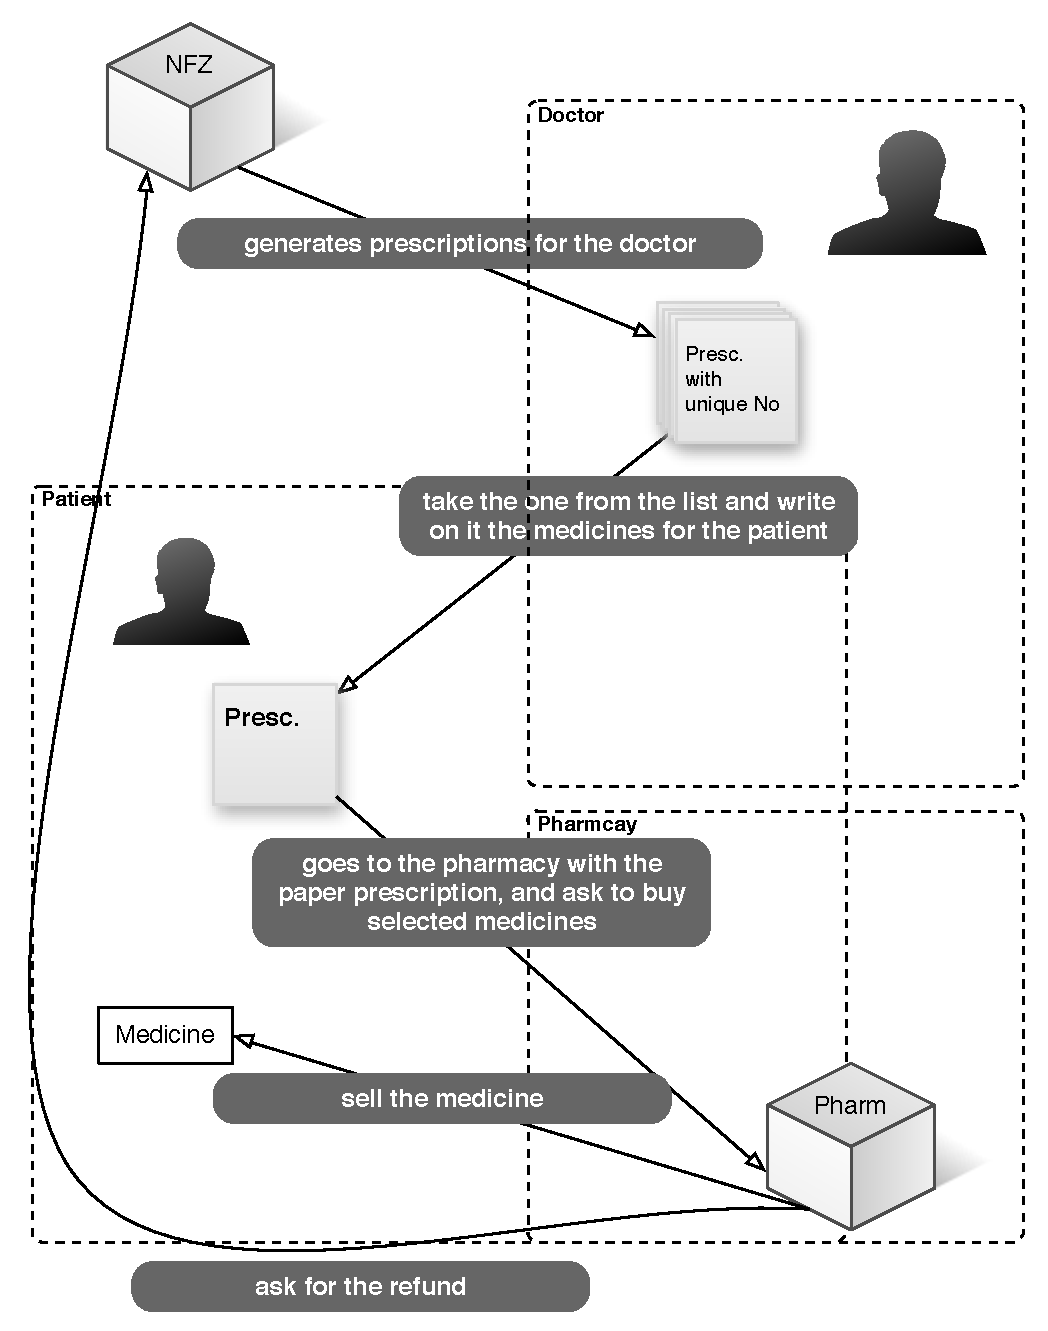
\includegraphics[scale=0.6]{cs.pdf}
    \caption{The main points of currently used system}
    \label{fig:mp_cs}
\end{figure} 

\chapter{\noun{Threats and Inconveniences}   }

The way prescriptions are currently processed is vulnerable to many threats, and brings many inconveniences. The most important ones are listed below.

\section{\noun{NFZ}}

\subsection{\noun{Defraudation}}

Significant amount of money is being defrauded from NFZ because the
current system does not verify if the patient himself has bought the
medicine or the pharmacists has made a false call for the medicine
having some patient's prescription, prepared by the doctor (who is
also a part of the defraudation scheme).

\section{\noun{Patient}}

\subsection{\noun{Losing a prescription}}
The patient can lose the prescription and he cannot buy the medicines,
even if they are life-saving, he has to go to the doctor again and
ask for the new prescription.

If someone finds lost prescription, he can buy this medicines; what is more, this person
can get to know, who takes which medicines and in this way, he can
get to know, what is wrong with the person described on the prescription.

\section{\noun{Pharmacy}}

\subsection{\noun{Refundation delay}}
The pharmacy has to wait long time to refund costs for the medicines
from NFZ.

\subsection{\noun{Prescriptions with mistakes}}
Prescription tend to contain mistakes which makes it useless. In this situation the patient has to go to the doctor again so it's fixed.

\section{\noun{System}}

\subsection{\noun{Prescription forgery}}
Patient can try to copy the prescription and try to buy the medicines
few times in different pharmacies.

\subsection{\noun{ Pretending that prescription was lost}}
Patient can claim that he has lost his prescription and ask the
doctor to give him another one. Then he can buy the medicines twice.

\chapter{\noun{System Goals}}

The main objectives of our new design of the prescription management system is to limit the impact of the threats listed in Chapter \ref{ti} and improve the usability of the current system.
It will meet each of following requirements:
\begin{enumerate}
\item Prescriptions will be digitalized.
\item Prescriptions will be hard to forge.
\item Doctors will not be able to create prescriptions without knowledge of patient.
\item Prescriptions will be realized only by users with right credentials.
\item Patients and doctors will be able to browse history of prescriptions.
\item System will be secured with most up-to-date measures.
\item System will provide anonymous big data statistics.
\end{enumerate}

\newpage
\section{\noun{Central Server Objectives}}

The central server will be the core component of the whole digital prescriptions system. Key features of the central server are:
\begin{itemize}
 \item storing data of patients, doctors and pharmacists,
 \item allowing doctors to create prescriptions,
 \item allowing doctors and patients to review history of created prescriptions,
 \item allowing patients to transfer the ownership of prescription in secure, controlable manner,
 \item allowing pharmacists to review prescriptions yet to be realized,
 \item allowing prescription realization only if patient will be present at this event,
 \item validating the signatures of each party,
 \item providing annonymous statistics.
\end{itemize}

\section{\noun{Pharmacy Module Objectives}}

The pharmacy module objectives are:
\begin{itemize}
\item  The patient has to be sure that his sensitive data is stored in a secure way, and unauthorized person cannot get to know anything about his medicines and illnesses. 
\item The pharmacist has to be sure that he sells the right medicines only for the right patient. 
\item The refund process should be quicker and easier. 
\item The possibility of making mistakes on the prescription should be eliminated. 
\item The number of defraudations should be significantly limited.
\end{itemize}

\section{\textsc{Patient Module Objectives}}

The patient's  module objectives are:
\begin{itemize}
\item Possibility to get prescriptions without leaving home.
\item Functionality of transferring prescription to another person's account.
\item Availability of prescription history for a doctor.
\item Possibility to browse the list of medicines, doctors and pharmacies.
\end{itemize}

The prescription system from the patient point of view is based on smart cards. 
Each patient has a unique card with ID and a pair of cryptographic keys used to create a signature. 
The system could be easily combined with electronic IDs, when they become available in Poland.

The benefit of our system is that the patient could get the prescription without leaving home. 
He could request medicines by calling the doctor, who would prescribe them and make available on patient's account. 
In order to decrease the refund fraud problem, the patient has to realize the prescription in pharmacy by himself. 
If he is unable to realize it, he would be able to transfer it onto another person's account. 
Realization of a transferred prescription would only be possible for the person designed by the patient. 
However, if the patient would like to change the designed person or make the prescription again available for him to realize, he would be able to cancel the transfer.

Both the patient and the doctor (with patient's permission) are able to browse all of the patient's previous prescriptions. 
It could be helpful to reduce possibility of interactions between drugs prescribed by different specialists. 
Also, doctors would not be able to abuse this functionality, because it would require the patient to insert his smart card into the terminal in doctor's office.

Patient is able to browse the list of medicines, doctors and pharmacies. 
Thanks to this, he could easily check the leaflet of the medicine, find the phone number to the doctor or check the opening hours of the pharmacy.





\lhead[]{\textit{Prescriptions management: Project }}
\part{\noun{Project}}
\chapter{\noun{The main objectives}   }

The main objectives of our new design of the pharmacy module is to limit the impact of the threats listed above and improve the user-friendliness. 

	\textbf{ The patient} has to be sure that his sensitive data is stored in a secure way, and unauthorized person cannot get to know anything about his medicines and illnesses. \textbf{The pharmacist} has to be sure that he sells the right medicines only for the right patient. \textbf{The refund process} should be quicker and easier. \textbf{The} possibility of making \textbf{mistakes} on the prescription should be eliminated. \textbf{The} number of \textbf{defraudations} should be significantly limited.







%---------------DATABASE
\lhead[]{\textit{Prescriptions management: Database }}
\part{\noun{Database}}

\chapter {\noun{Use cases}}
We define two groups of actors - clients like patients, doctors and pharmacists which benefit from the system on daily basis and third parties - administrators, analytic tools and goverment authorities which cope with the system on special ocassions.

\begin{figure}[h]
\centering
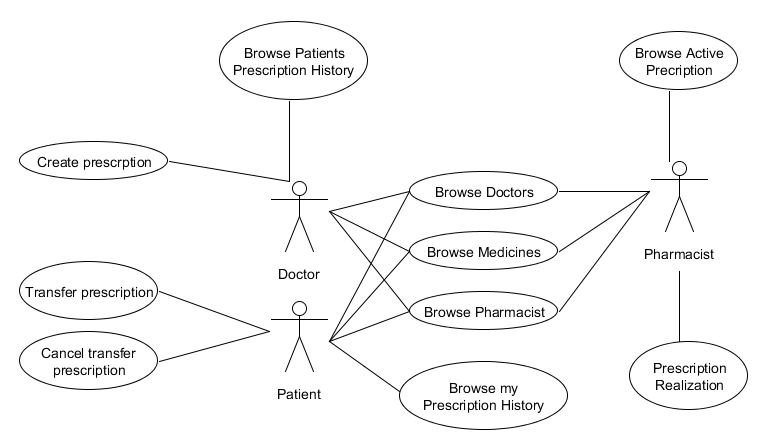
\includegraphics[width=1\textwidth]{database/standardUseCases.png}
\end{figure} 

Every use case requires the users to establish secure channel of communication with central server and have to be logged in which will be described more thorougly in section~\ref{sec:login}.
\section{Shared use cases}

Three use cases are applicable for patient, pharmacist and doctors and they consider browsing informations which can be publicly accessible, that is:
\begin{packed_enum}
\item Browse Doctors
\item Browse Medicines 
\item Browse Pharmacists
\end{packed_enum}
Rest of use cases which are applicable to only one actor is described in their respective subsections.
\small
\begin{longtable}{|p{6cm}|p{7.75cm}|}
   
    \hline
    Actors: Patient, Doctor, Pharmacist &Title: Browse Doctors \\ \hline
    Goal: & Allows to find doctor with specific name, address or license number. \\ \hline
    Scenario: & User enters any or all of name, address and license number of searched doctor. \\ \hline
    Result: & List of doctors corresponding to the query. \\ \hline
    Database  method: & \texttt{browse\_doctors} \\ \hline
    
\end{longtable}

\begin{longtable}{|p{6cm}|p{7.75cm}|}
    
    \hline
    Actors: Patient, Doctor, Pharmacist &Title: Browse Pharmacies \\ \hline
    Goal: & Allows to find pharmacist and pharmacy with specific name, address or license number. \\ \hline
    Scenario: & User enters any or all of name, address, license number of searched pharmacist or pharmacy name. \\ \hline
    Result: & List of pharmacists corresponding to the query. \\ \hline
    Database  method: & \texttt{browse\_pharmacies} \\ \hline

\end{longtable}


    \begin{longtable}{| p{6cm} | p{7.75cm} |}
    \hline
    Actors: Patient, Doctor, Pharmacist &Title: Browse Medicines \\ \hline
    Goal: & Allows to find medicine with specific name or type. \\ \hline
    Scenario: & User enters name or/and type of medicine he is searching. \\ \hline
    Result: & List of medicines corresponding to the query. \\ \hline
    Database  method: & \texttt{browse\_medicines} \\ \hline
    \end{longtable}

\normalsize

\section{\noun{Patient}}

\small
    \begin{longtable}{| p{6cm} | p{7.75cm} |}
    \hline
    Actors: Patient &Title: Transfer prescription \\ \hline
    Goal: & Allows to transfer a prescription to another patient and give him credentials to realize this prescription. Patient who transferred the prescription losses his right to realize it by himself. If he wants the prescription back he has to cancel the transfer (next use case). \\ \hline
    Scenario: & Patient enters his id, id of new owner, the prescription id he wants to transfer and his signature. \\ \hline
    Result: & OK response from database and iId of new owner of prescription. \\ \hline
    Database  method: & \texttt{transfer\_prescription} \\ \hline
\end{longtable}

    \begin{longtable}{| p{6cm} | p{7.75cm} |}
    \hline
    Actors: Patient &Title: Cancel Transfer Prescription \\ \hline
    Goal: & Allows to revert transfering of prescription to another patient. \\ \hline
    Scenario: & Patient enters his id, prescription id he wants transfers to revert and his signature. \\ \hline
    Result: & OK response from database. \\ \hline
    Database  method: & \texttt{cancel\_prescription\_transfer} \\ \hline
\end{longtable}

    \begin{longtable}{| p{6cm} | p{7.75cm} |}
    \hline
    Actors: Patient &Title: Browse My Prescriptions History \\ \hline
    Goal: & Patient can see his history of realized and created prescriptions.\\ \hline
    Scenario: & Patient sends his id which is signed by his key from smartcard. Patient can define the time span of returned prescriptions as also a filter to only return prescriptions which aren't realized yet. \\ \hline
    Result: & List of prescriptions for the patient. \\ \hline
    Database  method: & \texttt{browse\_prescription\_history} \\ \hline

\end{longtable}

\normalsize
\newpage
\section{\noun{Doctor}}

\small
    \begin{longtable}{| p{6cm} | p{7.75cm} |}
    \hline
   Actors:  Doctor &Title: Create prescription \\ \hline
    Goal: & Allows to create a new prescription in database for selected patient..\\ \hline
    Scenario: & Doctor enters his and patients ids, as well as the data specific to the medicine - id, dosage, unit and quanitity. Everything is signed by his key. \\ \hline
    Result: & OK response from database. \\ \hline
    Database  method: & \texttt{create\_prescription} \\ \hline
    \end{longtable}



    \begin{longtable}{| p{6cm} | p{7.75cm} |}
    \hline
    Actors: Doctor &Title: Browse Patients Prescriptions History \\ \hline
    Goal: & Doctor can see patient history of realized and created prescriptions..\\ \hline
    Scenario: & Doctor sends his id - he will see all prescriptions created by him. If he will add the id of patient with patients signature, he will see the full history of prescriptions of current patient. Doctor can define the time span of returned prescriptions as also a filter to only return prescriptions which aren't realized yet. \\ \hline
    Result: & List of prescriptions for the patient. \\ \hline
    Database  method: & \texttt{browse\_patient\_prescription\_history} \\ \hline
    \end{longtable}
\normalsize

\section{\noun{Pharmacist}}

\small
    \begin{longtable}{| p{6cm} | p{7.75cm} |}
    \hline
    Actors: Pharmacist &Title: Prescription realization\\ \hline
    Goal: & Pharmacist realizes the prescription. DB checks if the request can be verified and if the prescription is valid.\\ \hline
    Scenario: & Pharmacist enters his id, prescription id as well as drugs id, dosage and qunatity of medicine. Everything is signed by pharmacist key. \\ \hline
    Result: & OK response from database if operation was successful. \\ \hline
    Database  method: & \texttt{prescription\_realization} \\ \hline
    \end{longtable}



    \begin{longtable}{| p{6cm} | p{7.75cm} |}
    \hline
    Actors: Pharmacist &Title: Browse Active Prescriptions \\ \hline
    Goal: & Pharmacist can see prescriptions which are not yet realized. \\ \hline
    Scenario: & Pharmacist sends his id and id of current patient which are signed by both of their keys. Pharmacist can see only prescriptions which are not yet realized. \\ \hline
    Result: & List of prescriptions for the patient. \\ \hline
    Database  method: & \texttt{browse\_active\_prescriptions} \\ \hline
    \end{longtable}

\normalsize
\section{\noun{Special Users}}

There are also defined three other users which cope with the system on special ocassions.
These are - administrator, which maintains the system, analytic tools which can be used to obtain statistical data and the goverment authority which has super access to all the data after acquiring proper permissions from court or police.

\begin{figure}[h]
\begin{center}
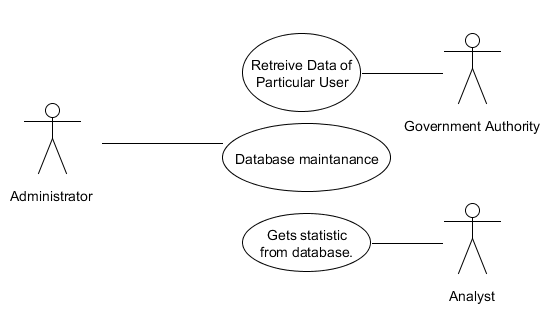
\includegraphics[width=0.7\textwidth]{database/specialUseCases.png}
\end{center}
\end{figure} 

\small
    \begin{longtable}{| p{6cm} | p{7.75cm} |}
    \hline
    Actor: Administrator &Title: Central Server maintenance \\ \hline
    Goal: & Administrator modifies the database, upgrades software etc. \\ \hline
    \end{longtable}


\newpage
    \begin{longtable}{| p{6cm} | p{7.75cm} |}
    \hline
    Actor: Goverment Authority &Title: Retreive Data Of Particular User \\ \hline
    Goal: & Goverment Authority (GA) can retreive all sensitive data of every user after showing permission to do so e.g. court order. GA account password can be separated into several pieces to ensure that one attacker won't be in possesion of the key. \\ \hline
    \end{longtable}



    \begin{longtable}{| p{6cm} | p{7.75cm} |}
    \hline
    Actor: Analytic tools &Title: Obtaining statistics from DB \\ \hline
    Goal: & Analyst can query the database for statistical data e.g. number of medicines sold in last month. Analyst can't query patients or link prescriptions data to particular person. \\ \hline
    \end{longtable}

\normalsize

\chapter{\noun{Communication}}
\begin{figure}[h]
\centering
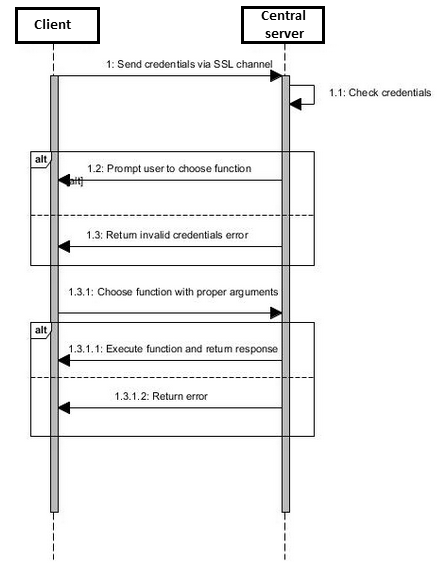
\includegraphics[width=0.7\textwidth]{database/sequence.png}
\caption{General communication diagram for patient, pharmacist and doctor}
\end{figure} 
Every communication with database can be described by one abstract scenario.
First central server and client establish session via SSL. After correct establishment of session, client chooses one of database functions that he can execute with appropriate arguments. Before using methods requiring signatures, client has to ask server for nonce, generated specially for the user. After obtaining the nonce, client can execute selected function.
Database verifies the correctness of signature and data passed in arguments and returns the result, or if one of the verification steps failed, error message.


\section{\noun{Connecting to Central Server}}\label{sec:login}
\begin{enumerate}
\item Enter smartcard with users private key and certificate (or establish paths to them)
\item set path of PostgreSQL to environment variable PATH.

\item in command line write $psql$ $'host=hosts_ip$ $port=port\_address$ $dbname=database\_name$ $user=username$ $sslmode=require$ $sslcert=user.crt$ $sslkey=user.key$ $sslrootcert=ca.crt'$ where:
	\begin{packed_enum}
	\item $host$ - IP of server where database is
	\item $dbname$ - is the name of database to which we want to connect
	\item $user$ - name of user which want to connect. Each part will have its own user name.
	\item $sslcert$ - certificate of user.
	\item $sslkey$ - private key of user.
	\item $sslrootcert$ - Certificate of CA.
	\end{packed_enum}
	Example login: $psql$ $'host=95.85.28.156$ $port=5432$ $dbname=PrescriptionSystemMk2$ $user=patient$ $sslmode=require$ $sslcert=patient.crt$ $sslkey=patient.key$ $sslrootcert=ca.crt'$
\item enter password
\end{enumerate}

\section{\noun{Nonces \& Verification Proccess}}

Randomly generated nonces are part of challenge-response protocol used in communication with database layer. Nonce are security measure against the replay attack. If a request require signature of any party, client has to ask database for generated nonce for given ID. After nonce is return, client has to:
\begin{enumerate}
 \item Conacatenate function name,
 \item function arguments,
 \item nonce.
 \item Calculate SHA-1 sum over the concatenated elements.
 \item Sign the with appropriate key\footnote{Signing method should be equal to invoking openssl command "openssl rsautl sign" with necessary parameters only}.
 \item Add the signature as the corresponding argument in function.
 \item Send the request.
\end{enumerate}

When the server obtains the request:

\begin{enumerate}
\item Takes users key from the database
\item Validates the signature
\item If the signature is validated, constructs SHA-1 sum in the same way as user
\item compares the verified, signed sum with one calculated in previous point
\item Executes the query if the sums are equal
\item Returns the result to the user
\end{enumerate} 

\clearpage
\begin{figure}[h]
\centering
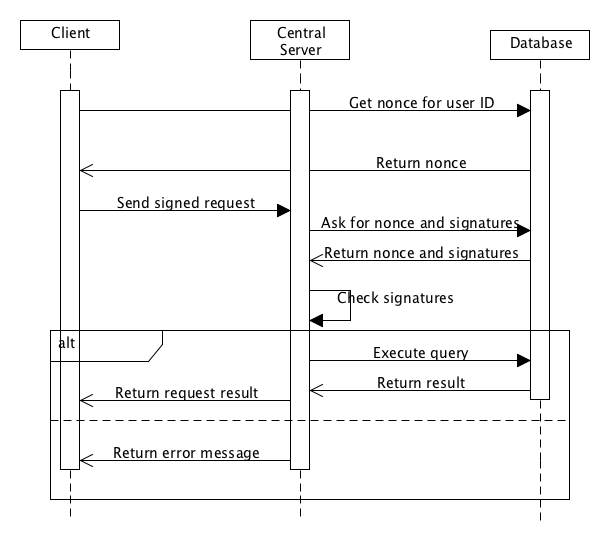
\includegraphics[width=0.8\textwidth]{database/nonce.png}
\caption{Sequence diagram of executing request with nonce signature}
\end{figure} 

\chapter{\noun{Database Functions and Schema}}

\section{\noun{Database Functions}}
After veryfing credentials sent by user to Central Server via SSL secure channel, user, depending on its role, will be able to execute set of functions, which will serve single purpose each (e.g. creation of new prescription).

\subsection{\noun{Shared Functions}}
%Browse medicines
\small
    \begin{longtable}{| p{3cm} | p{10.75cm} |}
    \hline
     & \texttt{browse\_medicines} \\ \hline
    Arguments: &  \begin{packed_enum}

    \item \texttt{name (string, optional, default = None)}
    \item \texttt{type (string, optional, default = None)}
	\end{packed_enum}        \\ \hline
    Usage: & Pharmacist sends his id and id of current patient which are signed by both of their keys. Pharmacist can see only prescriptions which are not yet realized. \\ \hline
    Result: & \begin{packed_enum}
    	\item \texttt{medicine\_id}
    	\item \texttt{name}
    	\item \texttt{prescription requirement}
    	\item \texttt{medicine type}
    	\item \texttt{maximum dosage}
    	\item \texttt{unit}
	\end{packed_enum}     \\ \hline	
    \end{longtable}

Note: Multiple records may be returned at single request.
%Browse doctors
    \begin{longtable}{| p{3cm} | p{10.75cm} |}
    \hline
     & \texttt{browse\_doctors} \\ \hline
    Arguments: &  \begin{packed_enum}
    	\item \texttt{name ( string, optional, default = None)}
		\item \texttt{address (string, optional, default = None)}
		\item \texttt{license\_number (string, optional, default = None)}

	\end{packed_enum}     \\ \hline
    Usage: & Entity using this function performs simple query which return all public data regarding registered doctors stored in DB. Arguments name, adress and license\_number narrows down result applying filters to the executed query. \\ \hline
    Result: & \begin{packed_enum}
    	\item \texttt{doctor\_id}
		\item \texttt{name}
		\item \texttt{address}
		\item \texttt{license\_number}
		\item \texttt{certificate}
		\item\texttt{ public\_key}
	\end{packed_enum}     \\ \hline	
    \end{longtable}

Note: Multiple records may be returned at single request.

\newpage
%Browse Pharmacies

    \begin{longtable}{| p{3cm} | p{10.75cm} |}
    \hline
     & \texttt{browse\_pharmacists} \\ \hline
    Arguments: &  \begin{packed_enum}
    	\item \texttt{pharmacist\_name ( string, optional, default = None)}
		\item \texttt{address (string, optional, default = None)}
		\item \texttt{license\_number (string, optional, default = None)}
		\item \texttt{pharmacy\_name (string, optional, default = None)}

	\end{packed_enum}     \\ \hline
    Usage: & Entity using this function performs simple query which return all public data regarding registered pharmacists stored in DB. Arguments name, adress and license\_number narrows down result applying filters to the executed query. \\ \hline
    Result: & \begin{packed_enum}
    	\item \texttt{pharmacist\_id}
		\item \texttt{name}
		\item \texttt{address}
		\item \texttt{license\_number}
		\item \texttt{certificate}
		\item \texttt{public\_key}
		\item \texttt{pharmacy\_name}
	\end{packed_enum}     \\ \hline	
    \end{longtable}
Note: Multiple records may be returned at single request.

\subsection{\noun{Patient Functions}}

%GetPatientNonce

    \begin{longtable}{| p{3cm} | p{10.75cm} |}
    \hline
     & \texttt{get\_patient\_nonce} \\ \hline
    Arguments: &  \begin{packed_enum}
    	\item \texttt{patient\_id (integer, mandatory)}
	\end{packed_enum}     \\ \hline
    Usage: & Function returns 1024 bit nonce for given patient\_id. \\ \hline
    Result: & \begin{packed_enum}
    	\item \texttt{nonce}
	\end{packed_enum}     \\ \hline	
			Comment: & New nonce is generated only if the last request was successfully verified.\\ \hline
    \end{longtable}


%Browse My Prescriptions History

    \begin{longtable}{| p{3cm} | p{10.75cm} |}
    \hline
     & \texttt{browse\_my\_prescriptions\_history} \\ \hline
    Arguments: &  \begin{packed_enum}
    	\item \texttt{patient\_id (integer, mandatory)}
		\item \texttt{executed (boolean, optional, default = None)}
		\item \texttt{start (date, optional, default = None)}
		\item \texttt{end (date, optional, default = None)}
		\item \texttt{patient\_signature (byte, mandatory)}
	\end{packed_enum}     \\ \hline
    Usage: & Patient requires history of his prescriptions. In order to get access to this kind of data, patient needs to sign his request using his secret key. Next, the signature will be veryfied by database. If signature will be acknowledged as genuine, database will return data about patient prescription history. Database provides patient the ability to filter his history by mean of time span and by the information about execution of prescriptions. \\ \hline
    Result: & \begin{packed_enum}
    	\item \texttt{prescription\_id}
    	\item \texttt{doctor\_id}
    	\item \texttt{doctor name}
    	\item \texttt{doctor address}
    	\item \texttt{doctor license number}
    	\item \texttt{prescription\_owner\_id}
    	\item \texttt{drug id}
    	\item \texttt{dosage}
    	\item \texttt{max dosage}
    	\item \texttt{unit}
    	\item \texttt{quantity}
    	\item \texttt{execution}
    	\item \texttt{time of execution}
    	\item \texttt{pharmacy\_id}
    	\item \texttt{pharmacy\_name}
    	\item \texttt{pharmacy\_adress}
	\end{packed_enum}     \\ \hline	
    \end{longtable}
Note: Multiple records may be returned at single request.

\newpage
%transfer_prescription

    \begin{longtable}{| p{3cm} | p{10.75cm} |}
    \hline
     & \texttt{transfer\_prescription}\\ \hline
    Arguments: &  \begin{packed_enum}
    	\item \texttt{patient\_id (integer, mandatory)}
    	\item \texttt{owner\_PESEL (integer, mandatory)}
		\item \texttt{prescription\_id (integer, mandatory)}
		\item \texttt{patient\_signature (byte, mandatory)}
	\end{packed_enum}     \\ \hline
    Usage: & Patient changes prescription owner to another patient, therefore allowing him to buy out specific prescription. It is important note, that after changing owner of prescription, original owner is NOT able to buy out his prescription until transfer is cancelled. \\ \hline
    Result: & \begin{packed_enum}
    	\item \texttt{new\_owner\_id}
		\item \texttt{"OK"}

	\end{packed_enum}     \\ \hline	
		Comment: & Prescription in database structure has two fields indicating prescription ownership - patientID (non-changeable, indicates the patient to which the medicine was prescribed) and owner\_PESEL (patient which will may realize the prescription).
		Transfering the right will only apply if both of these fields point to same id - thus we exclude the scenario when patients can pass the prescription to yet another person. After this operation the transferring patient losses right to realize the prescription - prevention from cloning the prescription.\\ \hline
    \end{longtable}


%Cancel prescription transfer

    \begin{longtable}{| p{3cm} | p{10.75cm} |}
    \hline
     & \texttt{cancel\_prescription\_transfer} \\ \hline
    Arguments: &  \begin{packed_enum}
    	\item \texttt{patient\_id (integer, mandatory)}
		\item \texttt{prescription\_id (integer, mandatory)}
		\item \texttt{patient\_signature (byte, mandatory)}
	\end{packed_enum}     \\ \hline
    Usage: & Patient changes actual owner of his prescription back to the original one (the patient himself) allowing him to buy out prescription and disallowing former owner of prescription to do so. \\ \hline
    Result: & \begin{packed_enum}
    	\item \texttt{"OK"}
	\end{packed_enum}     \\ \hline	
		Comment: & Prescription in database structure has two fields indicating prescription ownership - patientID (non-changeable, indicates the patient to which the medicine was prescribed) and ownerID (patient which will may realize the prescription). Cancelling will only work if patientID and ownerID are different and the signature over request is verified. \\ \hline
    \end{longtable}

\subsection{\noun{Doctor Functions}}

%get_doctor_nonce

    \begin{longtable}{| p{3cm} | p{10.75cm} |}
    \hline
     & \texttt{get\_doctor\_nonce} \\ \hline
    Arguments: &  \begin{packed_enum}
    	\item \texttt{doctor\_id (integer, mandatory)}
	\end{packed_enum}     \\ \hline
    Usage: & Function returns 1024 bit nonce for given doctor\_id. \\ \hline
    Result: & \begin{packed_enum}
    	\item \texttt{nonce}
	\end{packed_enum}     \\ \hline	
			Comment: & New nonce is generated only if the last request was successfully verified.\\ \hline
    \end{longtable}


%create_prescription

    \begin{longtable}{| p{3cm} | p{10.75cm} |}
    \hline
     & \texttt{create\_prescription} \\ \hline
    Arguments: &  \begin{packed_enum}
    	\item \texttt{doctor\_id (integer, mandatory)}
		\item \texttt{patient\_id (integer, mandatory)}
		\item \texttt{drug\_id (integer, mandatory)}
		\item \texttt{dosage (integer, mandatory)}
		\item \texttt{unit (integer, mandatory)}
		\item \texttt{quantity (integer, mandatory)}
		\item \texttt{doctor\_signature (byte, mandatory)}
	\end{packed_enum}     \\ \hline
    Usage: & Doctor prescribe single medicine to the patient, describing medicine, quantity and dosage. \\ \hline
    Result: & \begin{packed_enum}
    	\item \texttt{"OK"}
	\end{packed_enum}     \\ \hline	
		Comment: & Database does not requires patient signature to create a prescription for him - Prescription realization will require his key (thus his smartcard) so the medicine can't be bought without his knowledge. Also the doctor can create prescription without the need of meeting the patient face to face - which is and advantage for chronically ill patients.\\ \hline
    \end{longtable}


%browse_patient_prescription_history

    \begin{longtable}{| p{3cm} | p{10.75cm} |}
    \hline
     & \texttt{browse\_patient\_prescription\_history} \\ \hline
    Arguments: &  \begin{packed_enum}
    	\item \texttt{doctor\_id (integer, mandatory)}
		\item \texttt{patient\_id (integer, mandatory)}
		\item \texttt{start (date, optional, default = None)}
		\item \texttt{end (date, optional, default = None)}
		\item \texttt{bought(boolean, optional, default = None)}
		\item \texttt{doctor\_signature (byte, mandatory)}
		\item \texttt{patient\_signature (byte, optional)}

	\end{packed_enum}     \\ \hline
    Usage: & Doctor downloads patient prescription history. Doctor (unlike pharmacist) do not needs patient signature to browse history od prescription that he has created. If he wants the full history, patients signature is needed. \\ \hline
    Result: & \begin{packed_enum}
    	\item \texttt{prescription\_id}
    	\item \texttt{doctor\_id}
    	\item \texttt{doctor name}
    	\item \texttt{doctor address}
    	\item \texttt{doctor license number}
    	\item \texttt{prescription\_owner\_id}
    	\item \texttt{drug id}
    	\item \texttt{dosage}
    	\item \texttt{max dosage}
    	\item \texttt{unit}
    	\item \texttt{quantity}
    	\item \texttt{execution}
    	\item \texttt{time of execution}
    	\item \texttt{pharmacy\_id}
    	\item \texttt{pharmacy\_name}
    	\item \texttt{pharmacy\_adress}
	\end{packed_enum}     \\ \hline
	Comment: & If the patient signature is missing, database will only return prescriptions which were created by the doctor. If the patient signature is present and can be verified, doctor will receive the full history of patient. In case of any errors on verification, the request will be canceled. \\ \hline
    \end{longtable}
Note: Multiple records may be returned at single request.

\subsection{\noun{Pharmacist functions}}

%get_pharmacist_nonce

    \begin{longtable}{| p{3cm} | p{10.75cm} |}
    \hline
     & \texttt{get\_pharmacist\_nonce} \\ \hline
    Arguments: &  \begin{packed_enum}
    	\item \texttt{pharmacist\_id (integer, mandatory)}
	\end{packed_enum}     \\ \hline
    Usage: & Function returns 1024 bit nonce for given pharmacist\_id. \\ \hline
    Result: & \begin{packed_enum}
    	\item \texttt{nonce}
	\end{packed_enum}     \\ \hline	
			Comment: & New nonce is generated only if the last request was successfully verified.\\ \hline
    \end{longtable}

%prescription_realization

    \begin{longtable}{| p{3cm} | p{10.75cm} |}
    \hline
     & \texttt{prescription\_realization} \\ \hline
    Arguments: &  \begin{packed_enum}
    	\item \texttt{prescription\_id (integer, mandatory)}
		\item\texttt{ pharmacist\_id (integer, mandatory)}
		\item \texttt{drug\_id (integer, mandatory)}
		\item \texttt{unit (integer, mandatory)}
		\item \texttt{quantity (integer, mandatory)}
		\item \texttt{pharmacist\_signature (byte, mandatory)}
		\item \texttt{patient\_signature (byte, mandatory)}

	\end{packed_enum}     \\ \hline
    Usage: & Pharmacist will be able to realize patient prescription by pointing right prescription by giving its id, choose proper medicine (not necessairly the same as medicine prescribed by doctor, this check will be done by database), describe how many medicine is sold.\\ \hline
    Result: & \begin{packed_enum}
    	\item \texttt{"OK"}
	\end{packed_enum}     \\ \hline	
	Comment: & Request has to be signed by both patient's and pharmacist's keys. If the signature is incorrect, the database will return error message and the medicine shouldn't be given away.\\ \hline
    \end{longtable}


%browse_active_prescriptions

    \begin{longtable}{| p{3cm} | p{10.75cm} |}
    \hline
     & \texttt{browse\_active\_prescriptions} \\ \hline
    Arguments: &  \begin{packed_enum}
    	\item \texttt{pharmacist\_id (integer, mandatory)}
		\item \texttt{patient\_id (integer, mandatory)}
		\item \texttt{pharmacist\_signature (byte, mandatory)}
		\item \texttt{patient\_signature (byte, mandatory)}
	\end{packed_enum}     \\ \hline
    Usage: & Pharmacy is able to see all active (not bought) prescriptions of current patient, which agrees to show this data to the pharmacy by signing request. \\ \hline
    Result: & \begin{packed_enum}
    	\item \texttt{prescription\_id}
    	\item \texttt{doctor\_id}
    	\item \texttt{doctor name}
    	\item \texttt{doctor address}
    	\item \texttt{doctor license number}
    	\item \texttt{prescription\_owner\_id}
    	\item \texttt{drug id}
    	\item \texttt{dosage}
    	\item \texttt{max dosage}
    	\item \texttt{unit}
    	\item \texttt{quantity}
    	\item \texttt{execution}
    	\item \texttt{time of execution}
	\end{packed_enum}     \\ \hline	
		Comment: & If the signatures of patient or pharmacist are incorrect, database will return an error. If there are no non-realized prescriptions, database will return empty list.\\ \hline
    \end{longtable}
Note: Multiple records may be returned at single request.
\normalsize
\newpage
\section{\noun{Database schema}}

\begin{figure}[h]
\begin{center}
\includegraphics[width=1.07\textwidth, height=0.5\textheight , angle=90]{database/databaseSchema.png}
\end{center}
\end{figure} 

\chapter{\noun{Central Server Security Standards}}
\section{\noun{Physical Security}}
\begin{packed_enum}
	\item Servers is protected by backup and offsite data storage. The offsite storage of backup media is in a secure backup-vendor secure facility.
	\item A facility with Uninterruptible Power Supply (UPS) supporting all servers and essential peripheral equipment (console servers, etc).
	\item A facility with a climate controlled environment separate from the building HVAC, (dedicated air conditioning with in-room temperature controls).
	\item A facility with cooling and electrical capacity that is planned and monitored for outages.
	\item Secured access to the facility with documentation listing all individuals who currently have access and monitoring/auditing of ingress/egress via staff/video/etc.
	\item Servers in the facility must require authentication for local access (i.e. consoles are not left logged in while unattended).
	\item For facilities that use access codes, the capability to quickly change the access codes if personnel changes warrant is required.  Access codes must be changed at least annually.
	\item A facility with automated fire detection and suppression systems.
\end{packed_enum}



\section{\noun{Data Encryption}}

\begin{packed_enum}
	\item Hard disks, on which are stored databases, will be encrypted by external program TrueCrypt. TrueCrypt encrypts whole data on hard disk in real time. 
	\item Databases will be encrypted by TDE (Transparent Data Encryption). TDE encrypts:
        \begin{packed_enum}
			\item Database files
			\item Database Snapshots
			\item Transaction Log File
            \item Backups
		\end{packed_enum}
	using DEK ( Database Encryption Key ) which is protected by certificate.
\end{packed_enum}

\section{\noun{Backup Procedure}}
\begin{packed_enum}
	\item To ensure no data loss, database is replicated in real-time to a server in another location - this location meets conditions mentioned in section 5.1.
	\item Additionally, regular backups are made every day.
	\item Backups are kept for reasonable amount of time:
        \begin{packed_enum}
			\item Daily backups - 1 week
			\item Weekly backups - 1 month
			\item Monthly backups - 1 year
			\item Annual backups - forever
		\end{packed_enum}
	\item All backups are encrypted with measures described in section 5.2.
\end{packed_enum}

%----------------PHARMACY
\lhead[]{\textit{Prescriptions management: Pharmacy }}
\part{\noun{Pharmacy Module}}

\chapter{\noun{Environment Description and Data Flows}   }


All the pharmacies which will be using our system must have broadband internet access, two smart card readers and two terminals: one for a pharmacist and one for a customer. The terminals apart from displaying the data need to handle all the confirmation actions on both sides. \newline
Pharmacists and pharmacies’ customers need to have valid smart cards which store their identification data (names, surnames, PESEL numbers and digital certificates). All the certificates must be given by a defined certification authority and renewed when necessary.


\textbf{\noun{Scenario}}

\begin{enumerate}
  \item Customer inserts his card into the reader and enters PIN number.
  \begin{enumerate}
	\item System checks whether PIN is correct (if it is not, an appropriate message is displayed and the process cannot be continued).
  \end{enumerate}
  \item Terminal displays list of active prescriptions to both buyer and pharmacist.
  \item Buyer selects prescriptions to buy.
  \item Pharmacist inserts his card into his reader and authenticates himself to the system (assuming that the card is not already inserted).
  \begin{enumerate}
	\item  If authentication is not possible (eg. card of the pharmacist is invalid), an appropriate error message appears on the screen and the process can't be continued.
  \end{enumerate}
  \item The pharmacist marks prescriptions selected by the customers as 'to be bought'.
  \item System checks whether prescriptions have already been bought (in case someone tampers with the card).
  \item System verifies validity of prescriptions (expiration date, credentials of the doctor etc.)
 \begin{enumerate}
	\item If some prescriptions are invalid, an appropriate message appears on the screen and system marks the prescriptions as 'invalid'.
  \end{enumerate}
  \item  If the drug from the prescription is not available (or the buyer does not want it for some reason), pharmacist can instead sell a substitute. For that, he is able to write information about selling a substitute to the system.
  \item Buyer confirms the prescriptions to be bought (including possible substitute replacements).
  \item Pharmacist gives the drugs to the buyer, confirms the selling and the system marks the prescriptions as 'bought'.
  \item  Buyer takes the drugs and removes his card from the reader.
\end{enumerate}

 If before step 10 either card is removed from the reader, process is aborted and initial state of the prescriptions does not change.

\begin{figure}
    \centering
    \hspace*{-1.2in}
    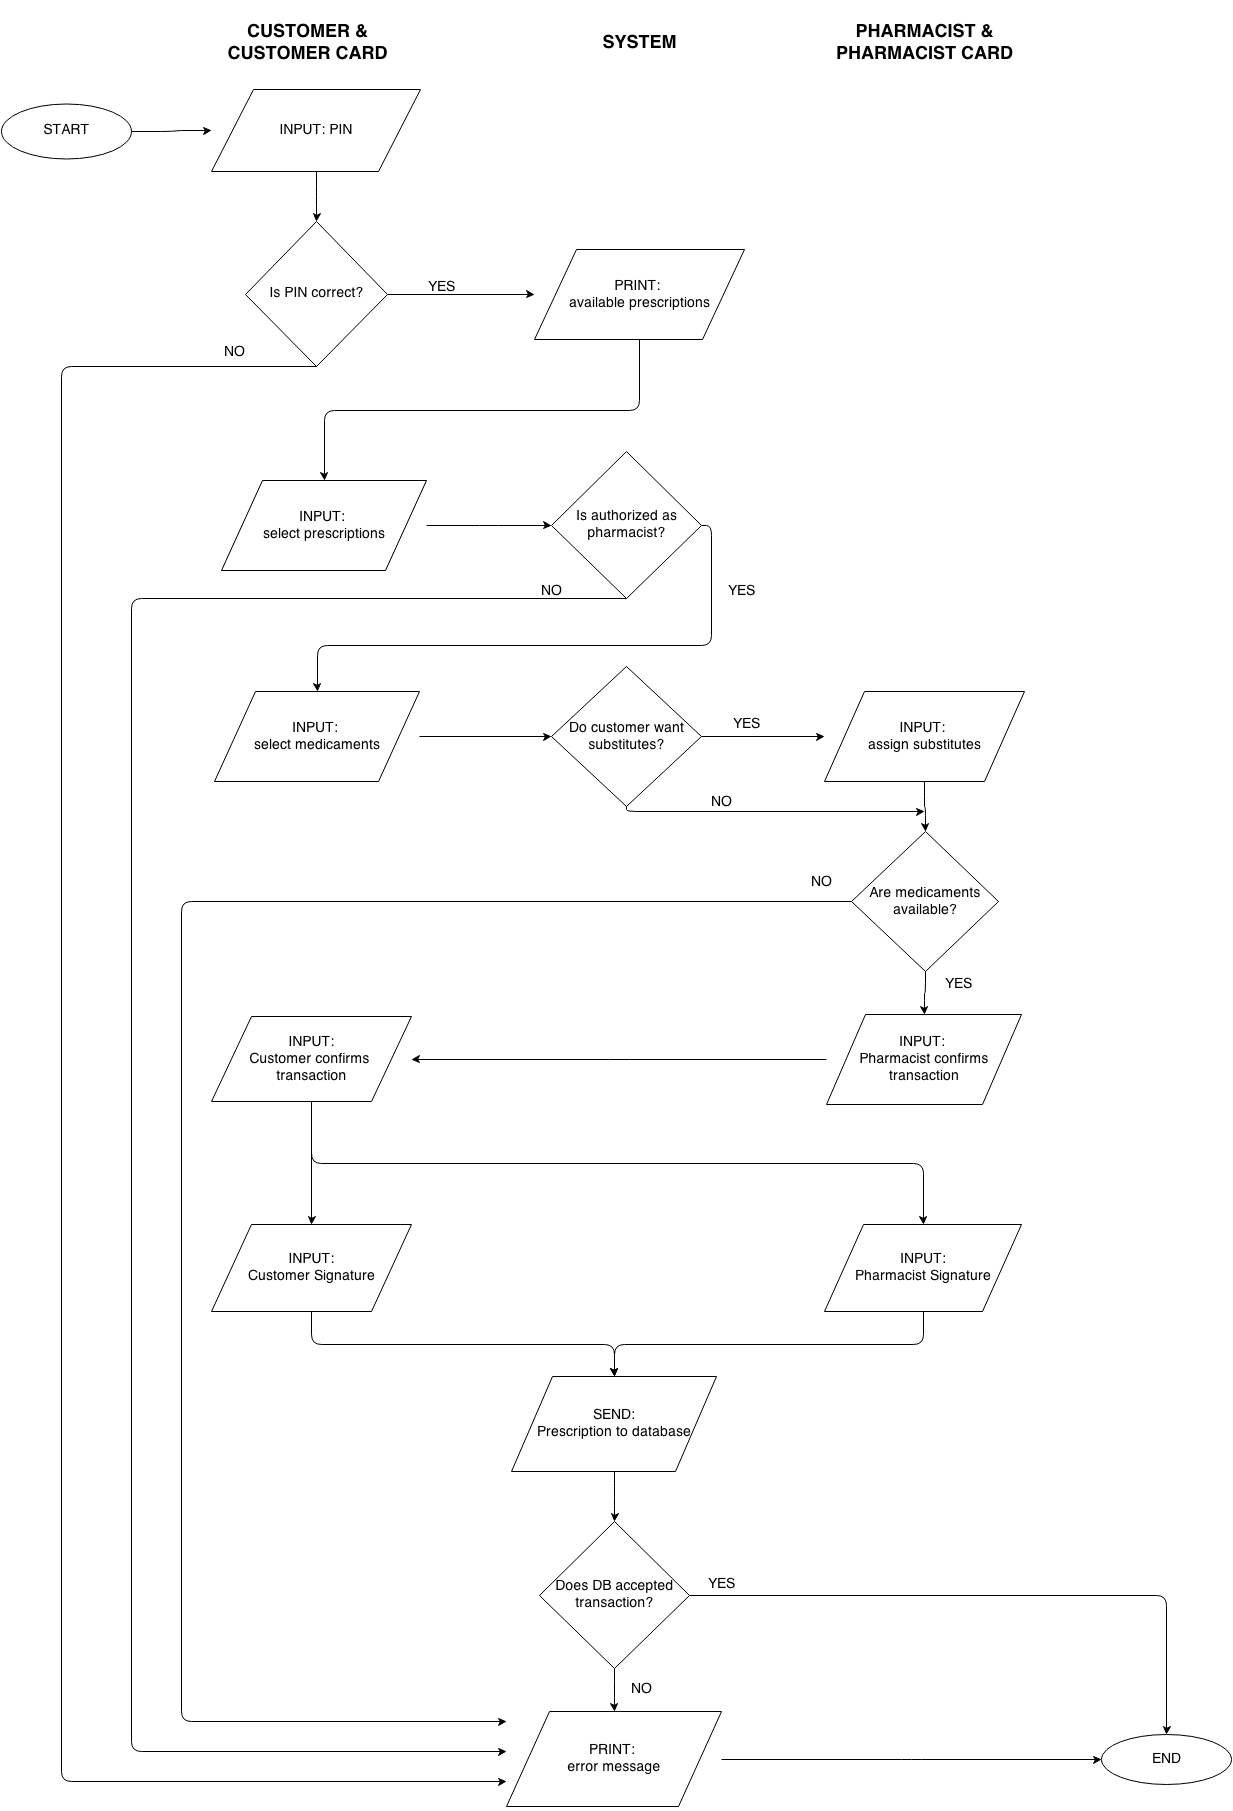
\includegraphics[width=0.98\textheight]{flow-chart.png}
    \caption{Flow chart}
    \label{fig:flowchart}
\end{figure} 


\chapter{\noun{Use cases}   }
In his chapter we present sequence diagram of the actions performed in the range of Pharmacy Module. Each step is detailed described. Not all actions are strongly required - sometimes it should depend on the security level requirement and budget possibilities. 

The first step is communication initialization. Actions performed in this step by the system elements are presented on the figure \ref{fig:s_q_step_1}
\begin{figure}	
	\hspace*{-1.5in}
    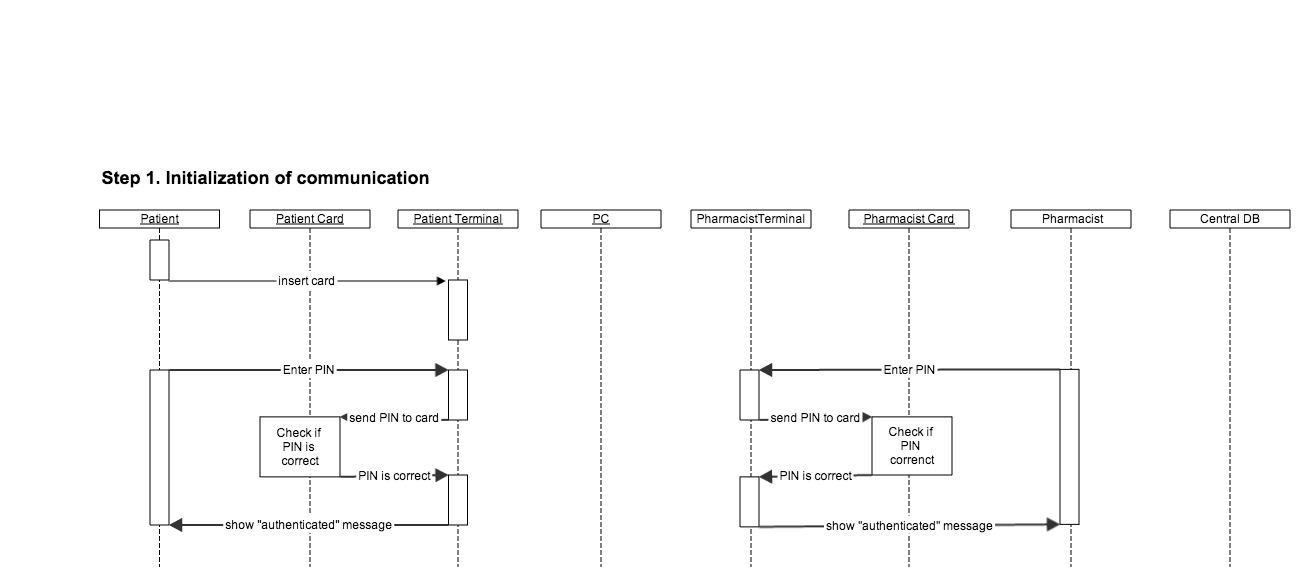
\includegraphics[scale=0.45]{s_d_1.png}
    \caption{Sequence diagram - step 1}
    \label{fig:s_q_step_1}
\end{figure} 

At the beginning, the patient put his personal card to the terminal and he enter the PIN as usual e.g. in the ATM. If the PIN is correct, the user can show appropriate message on the terminal screen. Also the pharmacist have to use his card and enter the PIN in the second terminal. Then, the system is ready to work. 

Necessity to use the PIN by the user and the pharmacist prevents the risk the situation, when e.g. the card was stolen or lost.


\begin{figure}	
	\hspace*{-1.5in}
    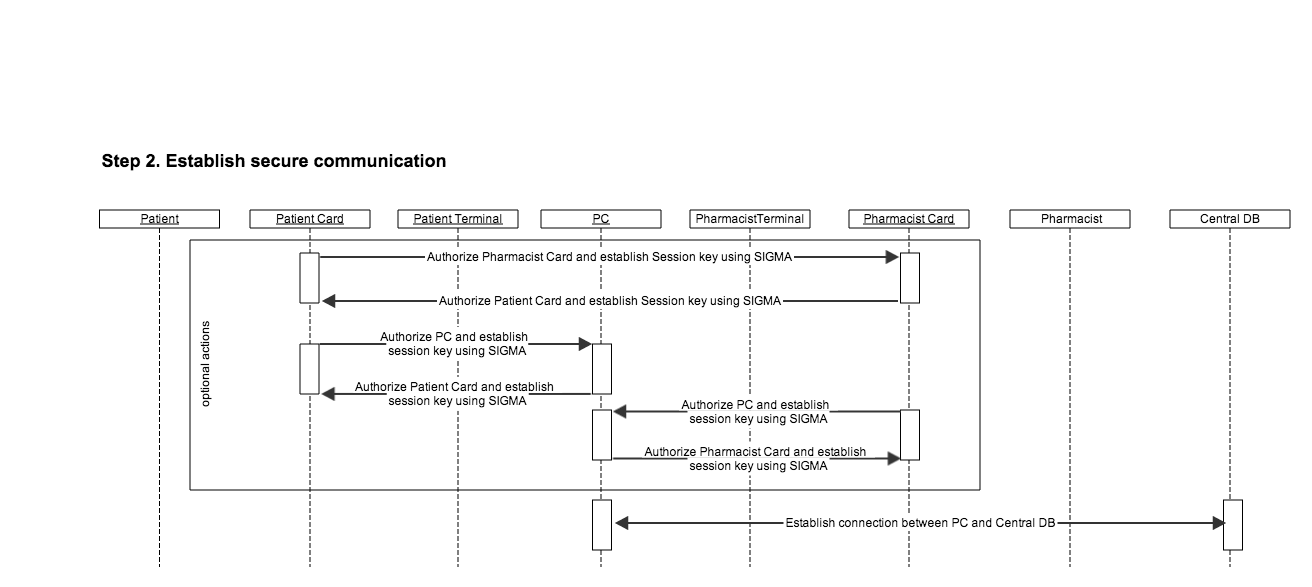
\includegraphics[scale=0.45]{s_d_2.png}
    \caption{Sequence diagram - step 2}
    \label{fig:s_q_step_2}
\end{figure} 

The second step, presented on the figure \ref{fig:s_q_step_2}, contains actions related with establishing secure communication ways between the system parties. There are marked the actions, which are optional and are not required for the system to work properly. Establishing secure communication between the cards allows the participant to be sure, that the patient ant pharmacist cards are not the fake cards and they are authenticated to each other.
Similarly, suing the SIGMA protocol between the card (patient or pharmacist) and the application installed on the PC, allows to authorization the application by the card and the card by the application. However. this two sub-steps can be implement, if the very-high level of the security from this point of view is required. 

\begin{figure}	
	\hspace*{-1.5in}
    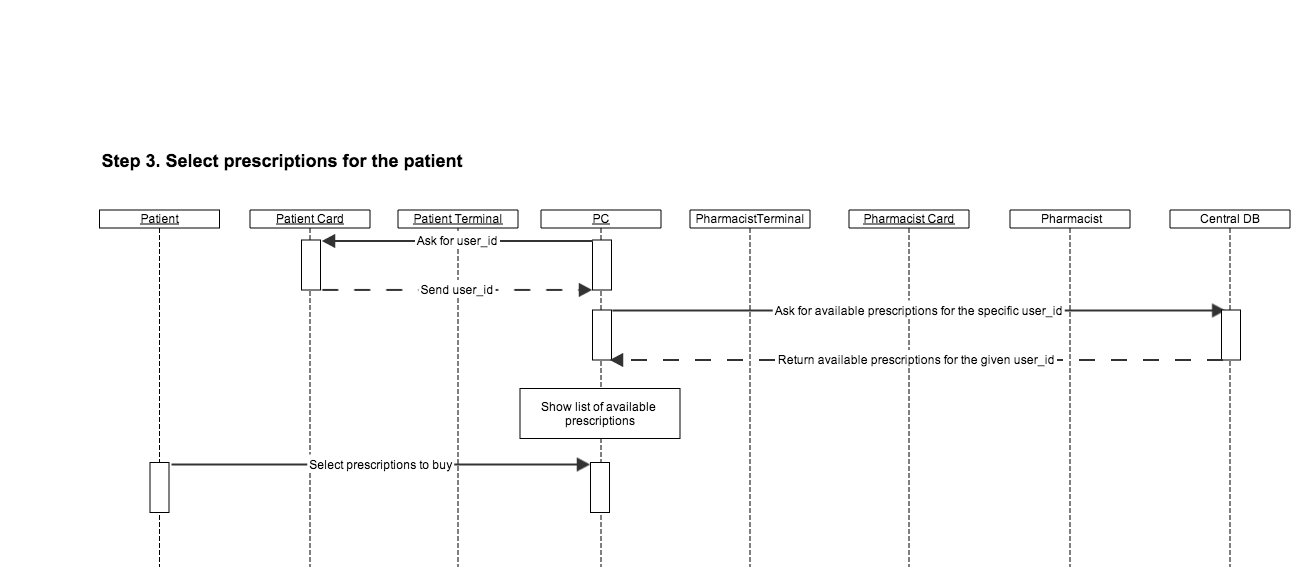
\includegraphics[scale=0.45]{s_d_3.png}
    \caption{Sequence diagram - step 3}
    \label{fig:s_q_step_3}
\end{figure} 

The figure \ref{fig:s_q_step_3} presents the point in the protocol, when the prescriptions for the user are download from the Central Database and are shown on the screen. Then, the patient have the possibility to select one or more of them to realize them. The data of the user are saved inside the patient card, so the application have to get this data to download appropriate prescriptions. 

\begin{figure}	
	\hspace*{-1.5in}
    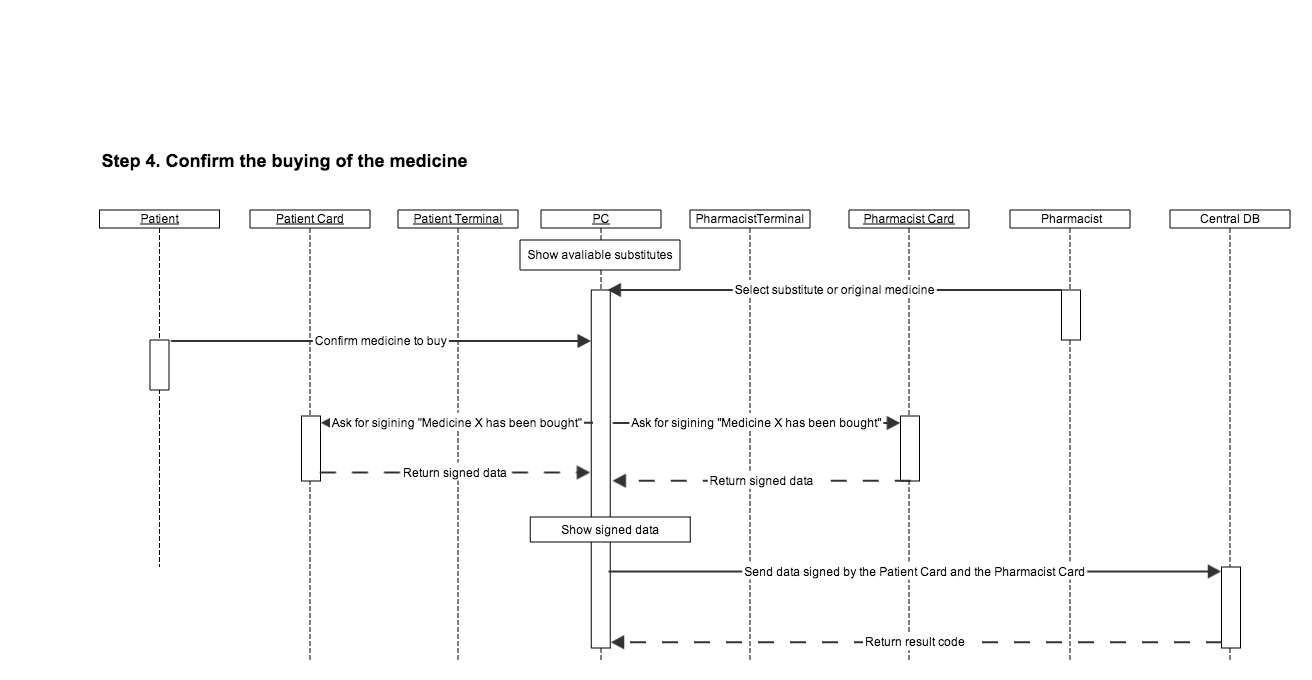
\includegraphics[scale=0.45]{s_d_4.png}
    \caption{Sequence diagram - step 4}
    \label{fig:s_q_step_4}
\end{figure} 




\lhead[]{\textit{Prescriptions management: Patient }}
%---------------PATIENT
\part{\noun{Patient}}
\lhead[]{\textit{Prescriptions management: Doctor }}
%---------------DOCTOR
\part{\noun{Doctor}}


%-----------------------------------------------------------
%\addcontentsline{toc}{chapter}{\numberline{}Bibliography}
%\include{biblio}
%-----------------------------------------------------------

%-----------------------------------------------------------
\end{document}
